\documentclass[titlepage]{article}
\usepackage{hyperref}
\usepackage{graphicx}
\graphicspath{ {../Diagrams/} }

% Title Page
\title{Real-time Trading Platform - Interim Report}
\author{John Costa - 100943301}
\date{06 Oct 2022 \\
  \\
  \Large{Final Year Project \\
Supervised By: Julien Lague \\
Royal Holloway, University of London}}

\begin{document}
\maketitle

\section{Introduction}
\subsection{The Problem}
For my final year project, I am creating a Real-time Trading platform, with a web interface and a robust backend, allowing the many users of the platform to trade - in real-time - with each other, with very low latency.

\subsection{Aims and Goals}
- Low latency
- Scalable
- Distributed
- Complex user actions on web interface
- Learn about it


\section{Research}
My primary source of information is the book \textit{Desining Data Intensive Application} ~\cite{kleppmann_2021}. This book provides an array of knowledge about building data intensive distributed applicatios that are reliable, scalable and usable.

\subsection{Architecture}
Modern systems tend to lean into a distributed architecture, meaning we have multiple services which communicate with each other, but are free to scale as load increases. It is unrealistic in the modern world to assume that all services will have the same amount of load and therefore could be packaged together, it is much more likely specific systems need to be scaled more, and perhaps other systems need to be scaled only at specific times of increased load. This means I need a more individual control over the multiple services that I wish to run. In my case, it is much more likely that looking at the top traded assets will be most of the load, therefore I need to scale the services which provides users with this information and have the information readily available on a cache, instead of fetching from permanent storage all time. 

\subsubsection{Microservices}
INCLDUE CITATION HERE FROM MICROSERVICE BOOK
Microservices are small, autonomous services that work together to form a complete system. Instead of creating a single application which has a single executable and database (Often refered to as a monolith), we break the system apart into services which all perform one thing, and do it well. These system then communicate with each other via a network (Most often the internet). \\

There are several advantages to using microserves:
\begin{itemize}
  \item Scalability: Each service can deside how many instances of it self it wants, this ties is really well with Docker which I talk about belo.
  \item Technological independance: We are not bound by technologies from other services, if we decide a service is better of with a certain database instead of another, we can make that decision. This also goes for programming languages.
  \item Resilience: If our system contains a singular monolith, there is a clear single point of failure. With microservices, if a system goes down - we lose functionality yes, but we do not lose the entire system as other services may still perform they functions.
\end{itemize}

However, this does make the entire development process more complex. We are no longer talking about a single application, but instead about developing multiple, smaller application that must all talk to each other flawlessly, with low latency and must allow for errors to occur in other services without the service itself going down.

\subsubsection{Docker}
Docker is an application which uses OS-level virtualization to deliver application in packages called containers. Docker containers do not include a Guest OS, and only contain the binaries and system libraries necessary to run the required application, leading to an increased performance, decrease container size and more portability across machines. Other virtualization technologies such as KVM INSERT REF HERE, require a host operating system in order to run the isolated environment, this means docker beats KVM in terms of performance in almost every regard (INSERT REF OF RESEARCH PAPER). To run containers, the host machine requires the docker engine, which acts as a sort of hypervisor. This makes docker extremely portable across machines, as the docker engine is not a full hypervisor and allows the host machine to run normally, as well as hosting the docker engine.

\subsubsection{Docker Containers}
A docker container is the packaged application, running on top of the docker engine. Containers are "Span up", from docker images which are made with Dockerfiles, these Dockerfiles describe the base image you are using (Ubuntu, Nodejs, Nginx, etc...), and allows you to copy, compile or do anything inside of this isolated environment. After these images are build, they can be ran and turned into containers. As mentioned before these containers only include the resources needed for the application to run, hence the performance improvements over full isolted, virtualized environments.

\subsubsection{Docker Swarm and Microservices}
Docker swarm is a native way to scale docker containers into thousand of notes. Docker swarm allows for a very easy way to create microservices. We can run our many services in a swarm which will deal with replication for us, therefore we have a better system resilience, but docker swarm also includes load balancing across these replicated instances, giving us better system performance and scalability. It also handles container restarts if any of them fail, and because of the nature of docker, these restarts are often less than a second (obviously depending on the size of the application).

\subsubsection{Docker Swarm vs Kubernetes}

\subsection{Advanced Web Development}
Over the years, we have put an increased amount of resposibility on websites. Today, websites are the default options for building applications which users interact with everyday. Because of this increased resposibility, developers have had to create frameworks for building web applications, which are reactive and responsive to user input, but also provide a performant experience for the end user.

\subsubsection{Web framework}
A web framework is a library that allows developers to build web application, by autonamically performing certain tasks such as updating parts of the websites UI. There are various web frameworks, ranging from server-side rendering framerworks (NextJS, Laravel), to client-side rendering applications (React, SolidJS), and this is what I will be using. \\

Most modern frameworks are written in JavaScript, which is an advantage because that is the only language the browser can read (Except for WASM). This advantage often makes the application faster, and much closer to the browser than other web frameworks such as Ruby on Rails, which is written (as the name suggests), in Ruby. \\

In order to allow developers to quickly build application, and for these applications to be scalable, many modern frameworks use a special syntax called JSX, which is an extension to JavaScript that allows the developer to write HTML-like code inside of their JavaScript files, this means that the markdown for a component lives together with the state of the application, making the component an entire standalone part of the application, which contains its own state, markdown and most often, styling too. \\

There are a few features that a web framework must have in order to be adequate for my use:
\begin{itemize}
  \item Reactivity: When new data comes into the application, or the user updates something in the UI, the application must reactively respond to thse changes, and show them to the user.
  \item Component Based: Building a website from scratch without a framework runs quickly into a modularity problem, where you cannot easily seperate different parts of the UI from another. Because of this the framework I use will need to seperate components into different Classes/Functions, which I can in turn split into multiple files and organise them in a file structure which works for me. These components must be able to control their own state as well as the way they appear in the application.
  \item Performance: My application's main consern is speed, the user must be able to see, act on and finish trades with other users with very little latency, this means the framework must be fast and have as little overhead as possible.
\end{itemize}

\subsubsection{React}
INSERT REF HERE
React is a library for building client side application using JavaScript, by seperating different parts of the UI into delcarative components which manage their own state and life-cycle. It updates the UI by using a virtual dom, which updated the real dom when there are changes in any component, meaning that the entire dom does not need to re-render when there is a singular change. \\

Even though React is trusted by many thousands of companies, and loved across the world I have decided to not use it in my project, mostly because of performance. React re-renders whole component when state updates, not only that but it has to re-render child components which can create a snow-ball effect where the entire application is re-rendered. It is hard to avoid this, to do so we have to employ memoization which react supports, but this means we need to write more code simply because React re-renderes everytime state is updated. \\

\subsubsection{SolidJs}
INSERT REF HERE

SolidJs is a client-side web framework, highly insipred by React, in fact programming with Solid is extremely similar to programming with React, which is a very big advantage for me because I have a lot of experience programming with React. However SolidJS beats most other webframeworks in terms of performance. INSERT REF HERE. This is mostly because it lacks a virtual dom, therefore component are rendered only once, however it maintains reactivity by making direct changes to the real DOM, when state changes, making massive improvements on performance because the whole component does NOT need to re-render, as it would in React. \\

There are some disadvantages of SolidJs, most of these come from the very reason that makes it good, the lack of a virtual dom. Because Solid, needs to update the real dom programmatically, you need to carefully understand how solid components actually re-render, otherwise the application might not update in some scenarios. \\

Even though Solid is generally harder than React because it does not re-render as often, its very developer friendly APIs and brutal performance, make it the obvious pick for a performance based project such as this.

\subsection{Building and bundling}
As mentioned above, most modern web frameworks (React and Solid included), use JSX. This is great for the developer as it leads to quicker development and more maintainable code, however browsers do not natively support this syntax, and therefore the entire application must go through a stage of transpilatoin (Taking the JSX into regular JavaScript), and then bundling the application into a few JavaScript files which contain all of the components of the application. Therefore, I must use a tool which both transpiles the code and allows me to build it into a bundled JavaScript file which my end users can then interact with.

\subsubsection{Webpack}
INSERT REF HERE
Webpack is the industry standard tool to perform these functions, it is written in JavaScript and takes your code and outputs bundled, transpiled JavaScript files. Webpack has extensive configuration which allows the developer to really specify what settings they want (What version of JavaScript do you need, what polyfills are necessary, etc...). Webpack also provides a development server, allowing me to quickly view my application without having to completely build it. \\

Webpack is great, but there are a few drawbacks. First of the webpack configuration is notoriously difficult to setup, there are many options to choose from and a lot of pre-exiting knowledge is needed is order to create a good webpack configuration. \\

Another drawback is that it is written in JavaScript. JavaScript is great for web application but for intense workloads such as bundling and transpilation, it has weaker performance than compiled languages, making the developer experience here, slower and often less pleasing.

\subsubsection{Vite}
INSERT REF HERE

Vite is a newer build tool, which provides transpilation, bundling and a development server. Vite uses various other tools to complete these tasks and brings them to the developer in a very easily configured tool. \\

Vite uses ESBuild to transpile and build the JavaScript code, ESBuild is written in Golang which is a compiled language, and therefore has performance improvements in the 100x compared to similar tools written in JavaScript. \\

Vite also uses ES Modules, which is a newer browser feature which allows JavaScript files to import and export from other JavaScript files natively, without needing to go through a bundling stage. This means that the Vite Development Server is the fastest amongst tools like it, because it uses ES Modules directly, meaning it only needs to transpile the JavaScript files, but does not need to bundle them. It also allows for Hot-module replacement, which means that when a component changes, you replace that singular component and leave the others unchanged, increasing development speed trastically, because you don't need to wait for a long build time each time you make a change. \\

Vite also integrates very easily with React, Solid, or most other JavaScript frameworks. Making it often a 5 second step to get started with Vite with any of these JavaScript frameworks.

\subsection{Typescript}
INSERT REF HERE
JavaScript is the language that browsers use to make websites reactive, paving the foundation for web applications, and most user-facing applications. However, as web applications grew in size and responsibility, it became harder to develop applications which interact with complex data, because JavaScript does not natively support types, as it is a dynamic language, you often don't know the type of something and must perform extra validation in order to make sure data is of the format you expect. \\

This is where Typescript comes in. Typescript is JavaScript with types, it extends Javascript by inclduing interfaces, type declarations and even classes, each with specific fields. This makes working with complex data much easier as the developer is able to know the format of the data, as well as when they have made a mistake with specific objects. \\

Typescript compilers down to regular Javascript, but the compiler is strict and will not compile if it detects type errors, avoiding many of the mistakes that web developers face when building web applications. It also makes the code base much more maintainable, due to other developers knowing exactly the shape of the data they are interacting with. \\

Vite uses ESBuild, which is a build tool written in Golang, in order to compile the Typescript down to Javascript. \\

\section{Objectives}
- Authentication
- Allow users to buy/sell assets
- Scale

Currently I have authentication working, I also have the basic features of allowing users to buy and sell pre-set assets on the platform. I have called this stage the PoC (Proof of concept), where I built the basic features, to get a solid, working foundation - but also because it only includes a subset of the features, I was able to build it fairly quickly and fail very quickly. Furthermore it made me learn.

\section{Designed Architecture}
One of my projects main goals is to have a scalable architecture, which can automatically scale depending on load from the end users, I needed to create a robust architecture, by splitting the project into smaller systems (microservices) which all work and communicate together.

My project is split into the following (micro) services:
\begin{itemize}
  \item Authentication - User authentication.
  \item Hub - Initial point of contact for users.
  \item Brain - Permanent storage and data management.
\end{itemize}

Each of these services has their own database, as to reduce the dependency on a shared database, therefore increasing the autonomy of each service and increasing scalability as it decouples each system from the others. Below I go into further detail on each of these systems, I have also included a system diagram.

\hspace*{-3cm}
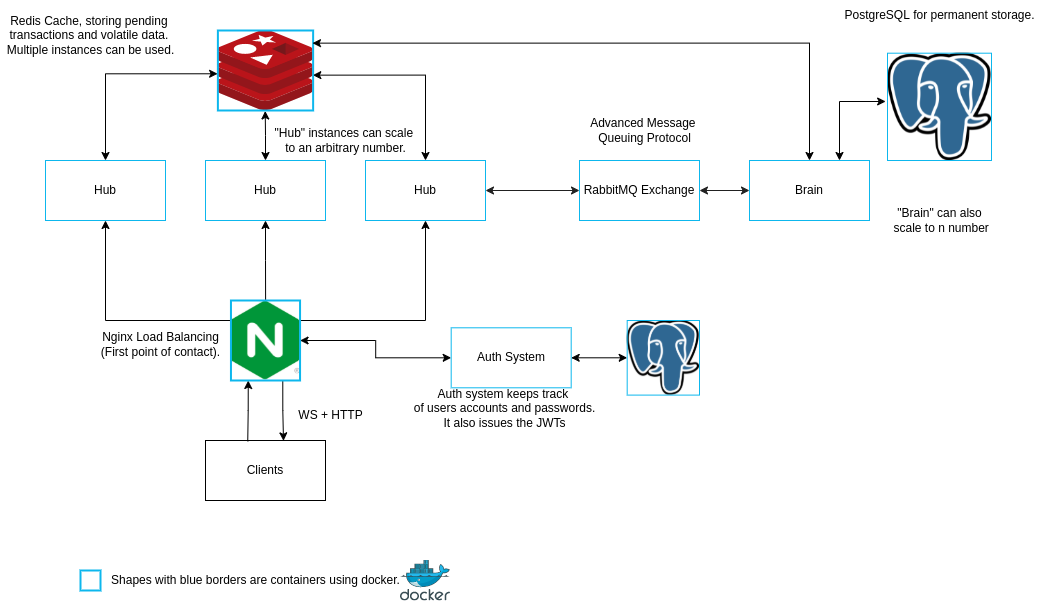
\includegraphics[width=1.5\textwidth]{Architecture.png}

\subsection{Authentication}
This system is the most isolated from the others. As you can see on the diagram is only communicates with the load balancer which comes straight from the user. This is because communication to and from the auth system contains very secure information such as passwords and access tokens, which if intercepted can allow users to access another users account. Therefore I don't want to handle this information for longer than I need to and definetly through the least number of systems possible - like this we go from the user to Nginx (A load balancer), straight to my authentication system. \\

The authentication system has its own database with a few tables that store user information. The database I choose is PostgreSQL, which as outlined in my plan, is one of the fastest, most robust and safest permaennt storage databases in the world, often outperforming competition by magnitudes or performance. The tables for this database are as follows: \\

TODO: Figure out how to make these nice
\begin{itemize}
  \item users
  \item userlogs
\end{itemize}

it includes 3 methods, and uses JWT, etc...

\subsection{Hub}
The hub is the only service without any permanent storage and this is very intentional. Its job is to act as a router for other services, but also a cache. My aim is to have this service serve from cache around 50 percent of the time. The hub communicates with a redis database which is a key pair in-memory database, which acts as a very fast caching system, that stores frequently requested data, as to avoid requesting this data from other systems. \\

The Hub can be vertically scaled very easily, together with the Redis database that it users, as Redis supports vertical scaling in a cluster mode. It is likely the system that will be scaled the most, as it will handle all of the users request (except for authentication).

\subsection{Brain}
A terrible name, but the Brain performs CRUD operations on the assets and transactions for the entire system, it acts as an API which the Hub can communicate with to fetch information from. The Brain like all other services has a database of its own, another PostgreSQL database. The Brain can also scale vertically just like all services but it's difficult to scale the PostgreSQL database vertically because it is difficult to split the data, instead a horizontal scaling approach will be required for the database portion of this service. \\

The brain also communicates with the Redis cluster which the Hub primarily interacts with. This is to update the cache so that the Hub can in future requests return data from this cache database instead of requesting the data from the Brain. The reason I do this step in the Brain service instead of on the Hub on return of the data, is because I want the Hub to only be conserned with handling user requests and either returning the data from cache, or handing it off to another service, as to not "Hold up the line". TODO: JUSTIFY THIS DECISONI WITH THE BOOK AND RESEARCH.

\subsection{Communication and Loadbalancing}
I have not yet described how these systems communicate with either one another or the user. To start with the user makes request to Nginx which can act as a very high performance web server, load balancer or reverse proxy. These requests are HTTP(s) requests (and also WS), and therefore this is what the Hub recieves from the user. \\

However, for the hub to communicate with the Brain service it does not use HTTP requests as these would be somewhat inefficient and not complex enough to handle some of the required distributed behavior of the systems, therefore I am using RabbitMQ to commuinicate between the Brain service and the Hub. RabbitMQ acts as a message exchange which supports AMQP (Advanced Messaging Queue Protocol), and with this I can create a sort of RPC (Remote Prodedural Call), from the Brain service. All whilst allowing many messages from multiple isntances of both services. \\

Microservices architectures generally have the problem of transmitting information across each other, efficiently. To mitigate this problem I have created a library which is shared across my multiple services, that includes the types for commonly used objects. This makes it much easier to share data across system because each one knows the shape of the data, and can easily encode it and decode it without many problems.

\section{Technologies used}
I have a variety of technologies for my project, these include frontend technologies to create a state of the art web interface, to backend technologies that allow the project to be scaled to as many users as it needs to be scaled to. \\

I have already talked about some of the technologies used. TODO: REFACTOR.

\subsection{Backend Technologies}
These are the technologies which I used to build the backend system, which consists of the Hub, Brain and Authentication. \\

\subsubsection{Golang}
As a programming language I have used Golang TODO: INSERT REF, it is a statically typed compiled language, known for its simplicity and ability to write extremely scalable systems, doing my own research I have found that a lot of modern architectures use Golang Real-time Trading Platform
John Costa - 100943301
06 Oct 2022
CS3821 - BSc Final Year Project
Supervised By: Julien Lague
Royal Holloway, University of Londonbecause of its stuff TODO: ADD REFS AND EXAND. \\

Golang also has an extremely fast compiler.

\subsubsection{PostgreSQL}
PostgreSQL is a relational database written in C, known for its performance and reliality. It uses SQL (Strucutured Query Language), to allow users to interact with the database. I have outlined the reason The reason I choose this database is because it consistently outperforms other databases (Both relational and non-relational), and performance is extremely important when building a system such as this one. However PostgreSQL does have limitation, such that it can only (easily), scale horizontally (Increasing the size of the machine), this is mostly due because the data is very centralized and highly linked in a relational database, but even with this big drawback, it still is the best, most performant option. To mitigate this drawback I have split the databases across the services, as to not have 1 central database, which would have been easier but would create a performance bottleneck. TODO: LOOK IN BOOK FOR REF.

\subsubsection{Redis}
Redis is an unstructured key-value pair in-memory database. Because it is in-memory, it is magnitudes faster than any persistent storage database, therefore I have used it as caching in my system, storing popular assets and data that is used frequently. \\
However, it is important that all the data stored in Redis, can be lost. This means I first have to store it in permanent storage, and only then store it for use in Redis. \\

The need for caching is extremely important in these systems. TODO: Further research on this.

\subsubsection{RabbitMQ}
TODO: RESEARCH ON MESSAGING SYSTEMS

\subsubsection{Gin - Golang HTTP Server}
A nice framework for building APIs using go.

\subsubsection{JWT}
JSON Web Tockets or JWTs for short, are cryptographically safe methods of client side authentication. A JWT is generated in the Authentication system, and signed with a private key, everytime the user wishes to authenticate themselves, they serve the JWT to any system, and if the signature on the JWT is correct then the user is authenticated, if not, we know the user either tampered with the signature or it isn't a valid JWT. JWTs can only encode a small amount of data in them, ranging from user information and ids, however this information is assessible to anyone who views the JWT, so it is important that the data is public knowledge. \\

I choose to use JWTs instead of cookie because they are very safe but still quite practicle. Like this I do not need to store cookies in the database and check everytime against a database that the user is logged in, reducing the amount of lookups various systems would have to perform.

\section{Software Engineering}

\subsection{Methodology}

\subsection{Project Management}
My project is quite complex and has a lot of moving parts which all have different criteria and different objectives. This will be a big challenge, so I will need to employ a good project management strategy if I want to keep on top of everything, and understand the complexity of my project.

For this I will use an app called Todoist TODO: REFERENCE HERE, which allows you to have Projects and labels, priorities and deadlines for various tasks. In Todoist (which I have used for a long time to manage almost everything in my life), I have implemented the system from Getting Things Done by David Allen TODO: REFERENCE HERE. This is a productivity/organisational system which involves splitting your tasks into lists and project, as well as review and process them in an appropriate maner.

\subsection{Version Control}

\subsubsection{Monorepo}
For this project, we were provided with 1 GitLab repo, however my project consists of various different services and parts that normally would not belong in the same repo. However, there is a common technique in industry of keeping all your code base in the same repository (monorepo), hence making CI (Contant Integration) and development easy, because everything is in one place and not scattered across multiple different project repositories. I am not using any monorepo management software although these do exist (Turborepo, Monorepo, Bazel), I keep my different projects stored in the apps TODO: Add formatting direcotry, hence seperating these somewhat, and each apps configuration files are stored in their corresponding folder, leaving the overall structure of the repository nice and clean.

\subsubsection{Bare repo and Worktrees}
Git has a feature called worktrees, this feature is not very well known, however I think it is a very powerful feature and one I have used through this project. Starting with cloning a barerepo, this means that we clone a Git Repository without cloning any of the files in the folder, with the main branch checked out. However, a bare clone just clones the .git file withotu any of the files, and we can use worktrees to edit various branches, worktrees are a way to have multiple branches in a git repository checked out at the same time, in seperate folders. This feature is very powerful because I was often working on 2 things at the same time (Frontend, backend and maybe the report), and naturally these live in different branches, therefore it is extremely useful to have them all checkout out at the same time. TODO: ADD REFERENCE FOR WORKTREES.

\subsection{Testing}



\subsection{Documentation}

\section{Assessment}

\bibliography{ref}
\bibliographystyle{plain}

\end{document}
